\let\negmedspace\undefined
\let\negthickspace\undefined
\documentclass[journal]{IEEEtran}
\usepackage[a5paper, margin=10mm, onecolumn]{geometry}
\usepackage{lmodern} % Ensure lmodern is loaded for pdflatex
\usepackage{tfrupee} % Include tfrupee package

\setlength{\headheight}{1cm} % Set the height of the header box
\setlength{\headsep}{0mm}     % Set the distance between the header box and the top of the text

\usepackage{gvv-book}
\usepackage{gvv}
\usepackage{cite}
\usepackage{amsmath,amssymb,amsfonts,amsthm}
\usepackage{algorithmic}
\usepackage{graphicx}
\usepackage{textcomp}
\usepackage{xcolor}
\usepackage{txfonts}
\usepackage{listings}
\usepackage{enumitem}
\usepackage{mathtools}
\usepackage{gensymb}
\usepackage{comment}
\usepackage[breaklinks=true]{hyperref}
\usepackage{tkz-euclide} 
\usepackage{listings}
\usepackage{gvv}                                        
\def\inputGnumericTable{}                                 
\usepackage[latin1]{inputenc}                                
\usepackage{color}                                            
\usepackage{array}                                            
\usepackage{longtable}                                       
\usepackage{calc}                                             
\usepackage{multirow}                                         
\usepackage{hhline}                                           
\usepackage{ifthen}                                           
\usepackage{lscape}
\usepackage{tikz}
\usepackage{tcolorbox}
\usetikzlibrary{matrix}
\usepackage{url}
\usepackage{xcolor}\begin{document}

\bibliographystyle{IEEEtran}
\vspace{3cm}

\title{10.4.3.5}
\author{EE24BTECH11005 - Arjun Pavanje}
% \maketitle
% \newpage
% \bigskip
{\let\newpage\relax\maketitle}
\textbf{Question:}
In a class test, the sum of Shefali's marks in Mathematics and English is $30$. Had she got $2$ marks more in Mathematics and $3$ marks less in English, the product of their marks would have been $210$. Find her marks in the two subjects. \newline
\solution \newline
Let $x, y$ be the marks obtained in Mathematics and English respectively. 
\begin{align}
  x + y = 30\\
  \brak{x+2}\brak{y-3} = 210
\end{align}
On combining the above two equations we get,
\begin{align}
  x^2 - 25x + 156
\end{align}
There are a few ways to solve this, \newline

\textbf{Newton Ralphson Method:}\newline
Start with an initial guess $x_0$, and then run the following logical loop,
\begin{align}
    x_{n+1} = x_n - \frac{f\brak{x_n}}{f^{\prime}\brak{x_n}} 
\end{align}
where,
\begin{align}
    f\brak{x} = x^2 - 25x + 156\\
    f^{\prime}\brak{x} = 2x - 25
\end{align}
The update equation will be
\begin{align}
	x_{n+1} = x_n - \frac{{x_n}^2 - 25x_n + 156}{2x_n - 25}\\
\end{align}
The problem with this method is if the roots are complex but the coeffcients are real, $x_n$ either converges to an extrema or grows continuously without any bound. 
In the case of complex solutions, we can just take our initial guess as a complex number, and that will return the required roots.
The output of a program written to find roots is shown below:
\begin{align}
  x = 12.000000000000014 \\
  x = 12.999999999999964
\end{align}
\textbf{Eigenvalue solution}\newline
For a polynomial equation of form $x_n+c_{n-1}x^{n-1}+\dots+c_2x^2+c_1x+c_0 = 0$ we construct a matrix called companion matrix of form
\begin{align}
  \myvec{
    0 & 0 & \cdots & 0 & -c_0\\
    1 & 0 & \cdots & 0 & -c_1\\
    0 & 1 & \cdots & 0 & -c_2\\
    \vdots & \vdots & \ddots & \vdots & \vdots\\
    0 & 0 & \cdots & 1 & -c_{n-1}\\
  }
\end{align}
The eigenvalues of the companion matrix are the roots of the polynomial equation. Thus, the quadratic equation and companion matrix are related by the characteristic polynomial equation. For the given question, the companion matrix comes out to be,
\begin{align}
  \myvec{0 & -156 \\ 1 & 25}
\end{align}
Using QR decomposition algorithm, we will now solve for the eigenvalues of the above companion matrix. \newline \newline Basic principle behind iterative QR decomposition is similar matrices.
Two square matrices $A$ and $B$ of size $n \times n$ are said to be $similar$ if there exists an invertible matrix $P$ such that:
\begin{align}
B = P^{-1} A P.
\end{align}
Similar matrices turn out to have the same eigenvalues. This can be easily proved,

Given that $A$, $B$ are similar matrices, and $P$ is an invertible matrix such that $B=P^{-1}AP$
By definition of eigenvalues,
\begin{align}
    \det(B-\lambda I)&=\det(P^{-1}AP -\lambda I)\\
    &=\det(P^{-1}AP -\lambda P^{-1}P)\\
    &=\det(P^{-1})\det(A-\lambda I)\det(P)\\
    &=\det(P^{-1}P)\det(A- \lambda I)\\
    &=\det(A-\lambda I)
\end{align}
Basic idea is to use similarity transforms to perform Schur Decomposition of matrix.
\begin{align}
  A = QUQ^{-1}
\end{align}
for some unitary matrix $Q$ (so that the inverse $Q^{-1}$ is also the conjugate transpose $Q^*$ 
of $Q$), and some upper triangular matrix $U$. The diagonal entries of the $U$ matrix are 
the eigenvalues. \newline
Steps to perform QR decomposition and accelerate its convergence,
\begin{enumerate}
\item \text{Convert to Upper Hessenberg form via Householder Reflections}
\item \text{Performing QR decomposition via Givens Rotations with shifts}
\item \text{Read off diagonal elements}
\end{enumerate}
Step 1: Performing Householder Reflections\newline
A square matrix A of order $n \times n$ is said to be in upper Hessenberg form if all the entries below the first subdiagonal are zero.
For example:
\begin{align}
H = \begin{bmatrix}
\times & \times & \times & \times \\
\times & \times & \times & \times \\
0 & \times & \times & \times \\
0 & 0 & \times & \times
\end{bmatrix}.
\end{align}
Applying QR decomposition to reach Schur-form to the matrix after it is in Upper Hessenberg form greatly accelerates rate of convergence.\\
Householder transformations are used to reduce a general matrix $A$ to Hessenberg form. A Householder reflector is an orthogonal matrix defined as:
\begin{align}
P = I - 2\textbf{uu}^{\top} \\
\end{align}
where $\|\textbf{u}\|=1$\\
If the entries of the matrix are complex, transpose is to replaced with conjugate transpose.
Vector $\textbf{u}$ must be carefully chosen such that the resultant matrix $P$ obtained from it must zero out all elements below the first subdiagonal for that particular column while maintaining similarity to preserve eigenvalues.
For a given column vector $x \in \mathbb{R}^n$, the vector $u$ is chosen as:
\begin{align}
\mathbf{u} = \frac{\mathbf{x} - \|\mathbf{x}\| \rho \mathbf{e_1}}{\|\mathbf{x} - \|\mathbf{x}\| \rho \mathbf{e_1}\|}
\end{align}
where:
\begin{itemize}
    \item $\mathbf{e_1}$ is impulse vector of appropriate dimensions, first element 1
    \item $\rho$ is something we have a degree of freedom in choosing as long as $|\rho|=1$
\end{itemize}
Usually, $\rho=-sign(x_1)$, but here for ease of calculation $\rho= -e^{j\phi}$ where $x_1=|x_1| e^{j\phi}$\\\\
We then construct Householder reflector matrix $P_1$ as,

\begin{align}
P_1 = \begin{bmatrix}
1 & 0 & 0 & 0 & 0 & 0 \\
0 & \times & \times & \times & \times & \times \\
0 & \times & \times & \times & \times & \times \\
0 & \times & \times & \times & \times & \times \\
0 & \times & \times & \times & \times & \times \\
0 & \times & \times & \times & \times & \times \\
\end{bmatrix} =
\begin{bmatrix}
1 & \mathbf{0}^{\top} \\
\mathbf{0} & I_5 - 2\mathbf{u_1 u_1}^{\top}
\end{bmatrix}
\end{align}
For a general case $P_i$ (for $i^{th}$ column) would be to create $I_{n-i} - 2u_i u_i^{\top}$ and expand it from the top left such that it is like an $n\times n$ identity matrix with it as the bottom right submatrix.\newline
Visualizing the process,
\begin{align}
\begin{bmatrix}
\times & \times & \times & \times \\
\times & \times & \times & \times \\
\times & \times & \times & \times \\
\times & \times & \times & \times
\end{bmatrix}
\xrightarrow{P_1}
\begin{bmatrix}
\times & \times & \times & \times \\
\times & \times & \times & \times \\
0 & \times & \times & \times \\
0 & \times & \times & \times
\end{bmatrix}
\xrightarrow{P_2}
\begin{bmatrix}
\times & \times & \times & \times \\
\times & \times & \times & \times \\
0 & \times & \times & \times \\
0 & 0 & \times & \times
\end{bmatrix}.
\end{align}
Step 2: Constructing Matrix for Givens Rotation \newline

A Givens rotation matrix $(G(i,j,\theta)$ zeroes out the element $a_{ij}$ by rotating in the $(i,j)$-plane. It is defined as:
\begin{align*}
G(i, j, \theta) = \begin{bmatrix}
1 & \cdots & 0 & \cdots & 0 & \cdots & 0 \\
\vdots & \ddots & \vdots & \ddots & \vdots & \ddots & \vdots \\
0 & \cdots & c & \cdots & s & \cdots & 0 \\
\vdots & \ddots & \vdots & \ddots & \vdots & \ddots & \vdots \\
0 & \cdots & -\overline{s} & \cdots & \overline{c} & \cdots & 0 \\
\vdots & \ddots & \vdots & \ddots & \vdots & \ddots & \vdots \\
0 & \cdots & 0 & \cdots & 0 & \cdots & 1
\end{bmatrix}
\end{align*}
where $\cos\theta$ and $\sin\theta$ are chosen such that the target element is eliminated.\\
To choose the values of $c$ and $s$ for the Givens rotation in QR decomposition, let $a_j$ be the element we wish to null out (i.e. make 0). Pick an arbitrary non-zero pivot element $a_i$ (on a different row). Usually, if we wish to null a particular sub-diagonal element, we pick the principal diagonal element above it as a pivot.
\begin{align*}
c = \frac{\overline{a_{i}}}{\sqrt{a_{i}^2 + a_{j}^2}}, \quad s = \frac{-\overline{a_{j}}}{\sqrt{a_{i}^2 + a_{j}^2}}
\end{align*}
Givens rotation essentially rotates the two rows that $a_i$ and $a_j$ are on such that $a_j = 0$ after rotation, other rows remain unaffected. 

These values rotate the vector formed by $a_{i}$ and $a_{j}$ to eliminate $a_{j}$ while maintaining the orthogonality of the rotation matrix. The choice of $c$ and $s$ ensures that the resulting transformed matrix has zeros below the diagonal in the desired locations.
Visualizing the process,
\begin{align}
\begin{bmatrix}
\times & \times & \times & \times \\
\times & \times & \times & \times \\
0 & \times & \times & \times \\
0 & 0 & \times & \times
\end{bmatrix}
\xrightarrow{G(3,2,\theta_1)}
\begin{bmatrix}
\times & \times & \times & \times \\
\times & \times & \times & \times \\
0 & 0 & \times & \times \\
0 & 0 & \times & \times
\end{bmatrix}
\xrightarrow{G(4,3,\theta_2)}
\begin{bmatrix}
\times & \times & \times & \times \\
\times & \times & \times & \times \\
0 & 0 & \times & \times \\
0 & 0 & 0 & \times
\end{bmatrix}.
\end{align}
After all Givens rotations, the resulting matrix is upper triangular:
\begin{align}
R = \begin{bmatrix}
\times & \times & \times & \times \\
0 & \times & \times & \times \\
0 & 0 & \times & \times \\
0 & 0 & 0 & \times
\end{bmatrix}.
\end{align}
For the Companion matrix in the given question,
\begin{align}
  c_k = \frac{0}{\sqrt{0^2 + 1^2}} = 0\\
  s_k = \frac{1}{\sqrt{0^2 + 1^2}} = 1\\
\end{align}
The sequence of Givens rotations $G_1, G_2, \dots, G_m$ satisfies:
\begin{align}
G_m \cdots G_2 G_1 A = R,
\end{align}
where \(R\) is upper triangular. The QR decomposition is obtained by combining the transposes of the Givens rotations into \(Q\):
\begin{align}
A = Q R, \quad Q = G_1^{\top} G_2^{\top} \cdots G_m^{\top}.
\end{align}
\begin{align}
    A_{k+1}&= R_k Q_k\\
    &=(G_n \dots G_2 G_1)A_k(G_1^{\top}G_2^{\top}\dots G_n^{\top})\\
    &= (G_n \dots G_2 G_1)A_k(G_n \dots G_2 G_1)^{\top}
\end{align}
Iteratively repeating this process causes the matrix to converge to upper triangular.\newline
Special Case: Jordan Blocks \newline

Jordan blocks are used to represent non-diagonalizable matrices. A Jordan block occurs when the Matrix on which eigenvalue alorithm is applied does not converge to Upper-Triangular. One example is when the enteries of the matrix are real, but they some of the eigenvalues are complex. Presence of a Jordan block indicates the presence of a pair of complex conjugate eigenvalues. 
\begin{center}
\begin{tikzpicture}
    \matrix[matrix of math nodes,
            nodes in empty cells,
            left delimiter={[},
            right delimiter={]}] (m) 
    {
        \times & \times & \times & \times & \times\\ 
        0      & \times & \times & \times & \times\\
        0      & \times      & \times & \times & \times\\ 
        0      & 0      & 0      & \times & \times\\ 
        0      & 0      & 0      & 0 & \times\\ 
    };

    \draw[red,thick] (m-2-2.north west) rectangle (m-3-3.south east);
\end{tikzpicture}
\end{center}
Jordan blocks can be handled by identifying where subdiagonal element is non-zero and solvinbg the $2 \times 2$ submatrix obtained.

Running the eigenvalue code for our companion matrix we get,
\begin{verbatim}
Eigenvalues:
(11.999964 + 0.000000i) 
(13.000036 + 0.000000i)\end{verbatim}
\begin{figure}[h!]
   \centering
   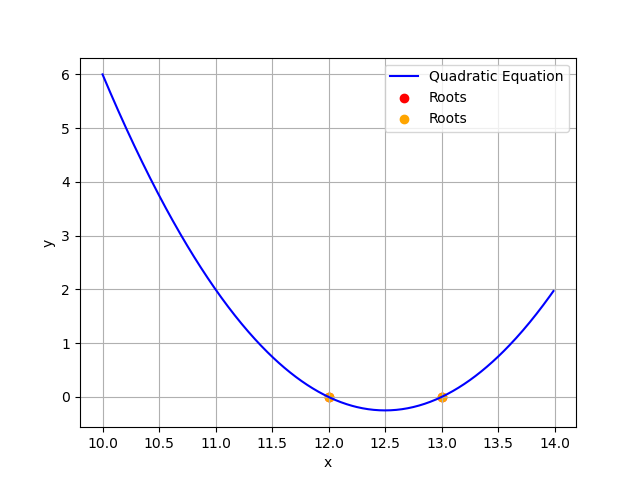
\includegraphics[width=1\columnwidth]{figs/fig.png}
   \caption{Solving quadratic equation $x^2 - 25x + 156$}
   \label{stemplot}
\end{figure}
\end{document}
